\begin{problem}[13]
作船舶润湿面积的量纲分析.
\end{problem}
% --------------------------------------------------------------------
\begin{solution}
\begin{minipage}[c]{0.8\linewidth}
船舶润湿面积$S$与船舶特征常度$l$, 排水体积$D$及行进速度$v$, 水的密度$\rho$及粘性系数$\mu$, 重力加速度$g$有关, 则有
\[
S = f(l,D; v; \rho, \mu, g)
\]
\end{minipage}
\begin{minipage}[c]{0.2\linewidth}
\begin{center}
\usetikzlibrary{calc,intersections,through,backgrounds}
\usetikzlibrary{decorations.pathreplacing,decorations.pathmorphing,arrows}
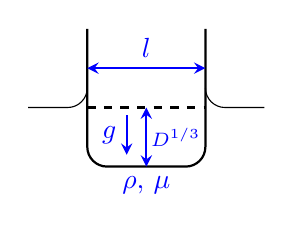
\begin{tikzpicture}
\draw [thick] (-0.75,1)--(-0.75,-0.5) arc(-180:-90:0.25)--(0.5,-0.75) node[below,midway,blue]{$\rho$, $\mu$} arc(-90:0:0.25) -- (0.75,1);
\draw[thick,blue,<->,>=stealth] (-0.75,0.5)--(0.75,0.5) node[above, midway]{$l$};
\draw[thick,dashed] (-0.75,0)--(0.75,0);
\draw (-1.5,0)--(-1,0) arc(-90:0:0.25) (1.5,0)--(1,0) arc(270:180:0.25);
\draw[thick,blue,->,>=stealth] (-0.25,-0.1)--(-0.25,-0.6) node [left,midway]{$g$};
\draw[thick,blue,<->,>=stealth] (0,0)--(0,-0.75) node [right=-2pt,midway,font=\scriptsize]{$D^{1/3}$};
\end{tikzpicture}
\end{center}
\end{minipage}\vspace{5pt}
上式中的各物理量的量纲分别为: $[S]=L^2$, $[l]=L$, $[D]=L^3$, $[v]=LT^{-1}$, $[\rho]=ML^{-3}$, $[\mu]=ML^{-1}T^{-1}$, $[g]=LT^{-2}$. 取$l$, $v$, $\rho$作为基本量, 且作为本问题的单位系统, 用以度量问题中的各量, 于是上式转化为
\[
\frac{S}{l^2} = f\bigg(1,\frac{D}{l^3};1,1,\frac{\mu}{\rho v l}, \frac{g}{v^2/l}\bigg)
\quad\Longrightarrow\quad
S = l^2 f\bigg(\frac{D^{1/3}}{l}, \frac{\rho v l}{\mu}, \frac{gl}{v^2}\bigg) = l^2 f(\Psi, \mathrm{Re}, \mathrm{Fr})
\]
其中无量纲数$\Psi$是几何长度之比, 反映相对载重量; $\mathrm{Re}$为雷诺数; $\mathrm{Fr}$为弗劳德数.
\end{solution}
